\documentclass[12pt,a4paper]{article}
\usepackage[utf8]{inputenc}
\usepackage[T2A]{fontenc}
\usepackage[english,russian]{babel}
\usepackage{amscd}
\usepackage{array}
\usepackage[dvips]{graphicx}
\usepackage{longtable,wrapfig}

\usepackage{amsfonts}
\usepackage{amsmath}
\usepackage{amssymb}
\usepackage{amsthm}
\usepackage{float}
\usepackage{mathrsfs}
\usepackage{colonequals}
\usepackage[font=small,labelfont=bf]{caption}
\usepackage[left=1in,right=1in,bottom=1in,top=1in]{geometry}
\usepackage[pdfpagelabels,hyperindex,colorlinks=true,linkcolor=blue,urlcolor=magenta,citecolor=green]{hyperref}
\usepackage{setspace}
\linespread{1.7}
\emergencystretch=1em

%% footnote definition begins
\makeatletter
\def\keywords{\xdef\@thefnmark{}\@footnotetext}
\makeatother
%% footnote definition ends

\newtheorem{thm}{Theorem}[section]
\newtheorem{cor}[thm]{Corollary}
\newtheorem{lem}[thm]{Lemma}
\newtheorem{examp}[thm]{Example}

\numberwithin{equation}{section}

\title{LaTeX шаблон на русском}
\date{} %leave it blank, looks better
\author{Петро Колосов}

\hypersetup{
    pdftitle={LaTeX шаблон на русском},
    pdfsubject={
        Your Subject List
    },
    pdfauthor={Петро Колосов},
    pdfkeywords={
        Your Keywords list
    }
}

\begin{document}
    \maketitle

    \begin{abstract}
        Lorem ipsum – псевдо-латинский текст, который используется для веб дизайна, типографии, оборудования,
и распечатки вместо английского текста для того, чтобы сделать ударение не на содержание,
а на элементы дизайна.
    \end{abstract}

    \keywords{2010 \emph{Mathematics Subject Classification.} Primary ..; Secondary \dots}
    \keywords{\emph{Key words and phrases.} Ключевое слово 1, Ключевое слово 2 \dots}
    \keywords{\emph{Website.} \href{https://kolosovpetro.github.io/}{\texttt{https://kolosovpetro.github.io}}}


    \section{Введение} \label{sec:introduction}
    \begin{equation}
    \frac{1}{2\pi i}\oint_{\gamma} \frac{f(z)}{z-z_0} \,dz = \sum_{n=0}^{\infty} \frac{f^{(n)}(z_0)}{n!}(z-z_0)^n\label{eq:equation}
\end{equation}

Текст статьи.
Пример цитирования~\cite{kolmogorov1950osnovnye, kolmogorov83kobminatorniye, GithubSource_2022, Sloane_theencyclopedia}.
Lorem ipsum – псевдо-латинский текст, который используется для веб дизайна, типографии, оборудования,
и распечатки вместо английского текста для того, чтобы сделать ударение не на содержание,
а на элементы дизайна.
Такой текст также называется как заполнитель.
Это очень удобный инструмент для моделей (макетов).
Он помогает выделить визуальные элементы в документе или презентации, например текст, шрифт или разметка.
Lorem ipsum по большей части является элементом латинского текста классического автора и философа Цицерона.
Слова и буквы были заменены добавлением или сокращением элементов, поэтому будет совсем неразумно пытаться передать содержание;
это не гениально, не правильно, используется даже не понятный латинский.
Хотя Lorem ipsum напоминает классический латинский, вы не найдете никакого смысла в сказанном.
Поскольку текст Цицерона не содержит буквы K, W, или Z, что чуждо для латинского, эти буквы, а также многие другие
часто вставлены в случайном порядке, чтобы скопировать тексты различных Европейских языков, поскольку диграфы
не встречаются в оригинальных текстах.

В профессиональной сфере часто случается так, что личные или корпоративные клиенты заказывают, чтобы публикация была
сделана и представлена еще тогда, когда фактическое содержание все еще не готово.
Вспомните новостные блоги, где информация публикуется каждый час в живом порядке.
Тем не менее, читатели склонны к тому, чтобы быть отвлеченными доступным контентом, скажем, любым текстом, который
был скопирован из газеты или интернета.
Они предпочитают сконцентрироваться на тексте, пренебрегая разметкой и ее элементами.
К тому же, случайный текст подвергается риску быть неумышленно смешным или оскорбительным,
что является неприемлемым риском в корпоративной среде.
Lorem ipsum, а также ее многие варианты были использованы в работе начиная с 1960-ых, и очень даже похоже,
что еще с 16-го века.

\begin{thmrus}
    Пример теоремы на русском языке.
\end{thmrus}

\begin{lemrus}
    Пример леммы на русском языке.
\end{lemrus}

\begin{thm}
    Example of theorem in english
\end{thm}

Пример изображения
\begin{figure}[H]
    \centering
    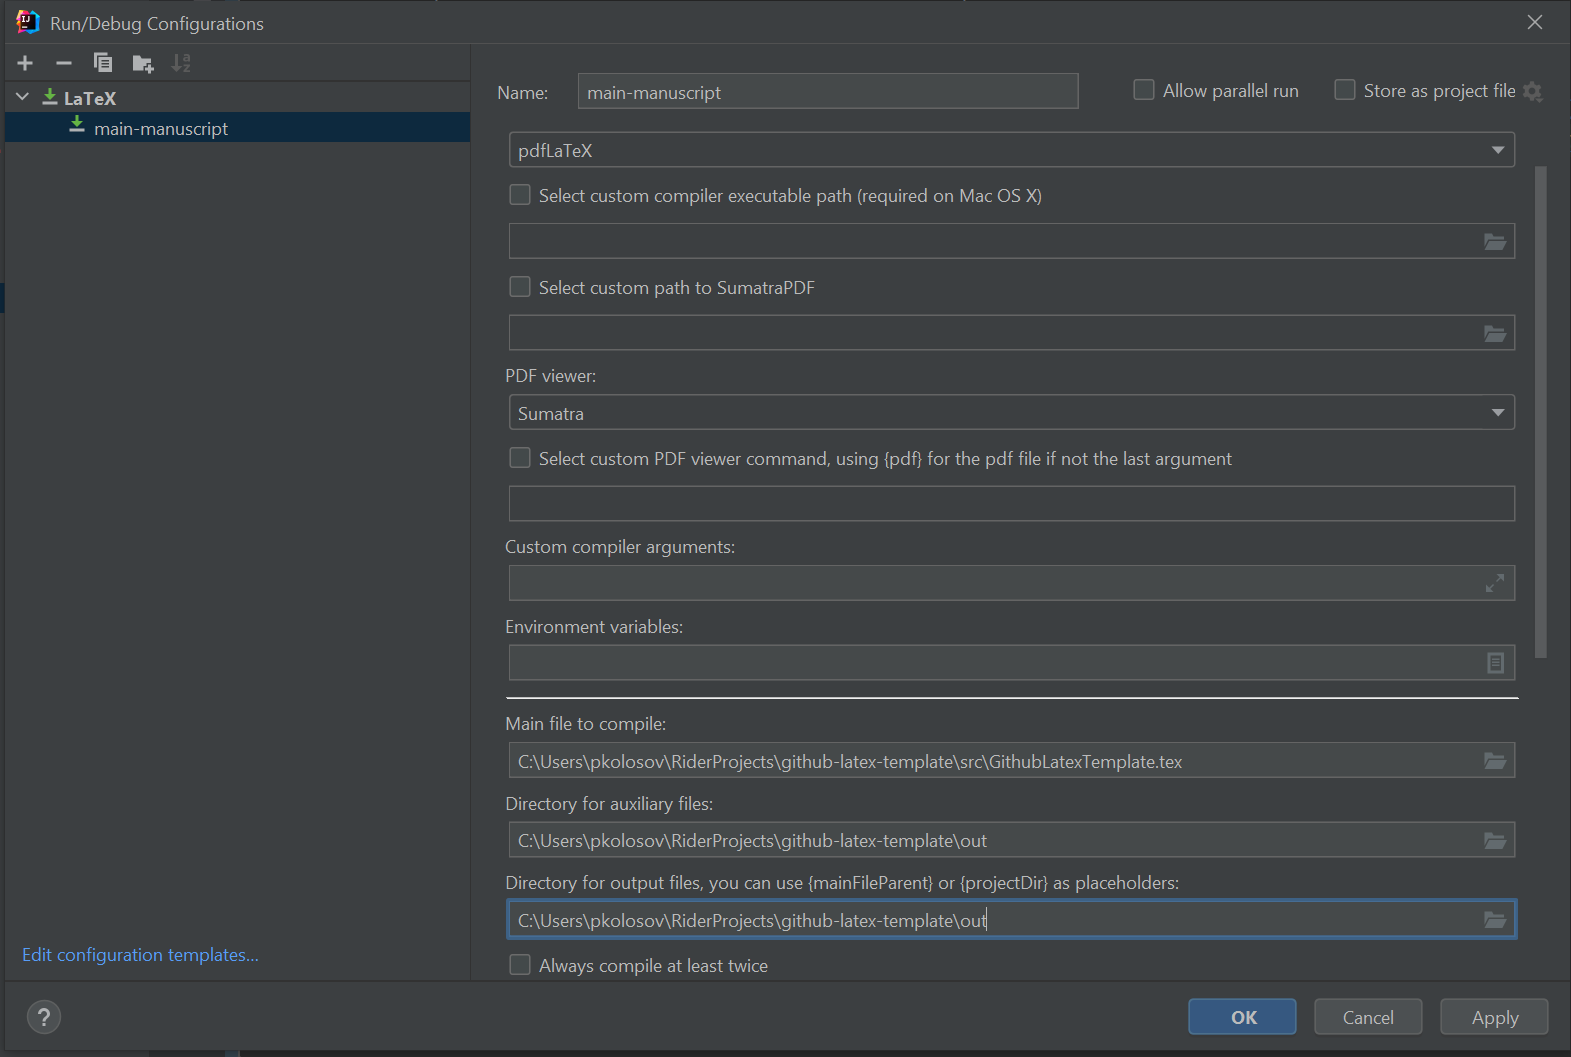
\includegraphics[width=0.8\textwidth]{../img/latex_configuration}
    ~\caption{Пример изображения.}\label{fig:figure}
\end{figure}

\begin{equation*}
    \llceil \nobarfrac{a}{b} \rrfloor_{m}
\end{equation*}
\begin{equation*}
    \llceilCoefficient{a}{b}{m}
\end{equation*}

And for any natural $m$ we have polynomial identity
\begin{equation}
    x^m = \sum_{k=1}^{m} T(m, k) \centralFactorial{x}{k}\label{eq:knuth-power-identity}
\end{equation}
where $\centralFactorial{x}{k}$ denotes central factorial defined by
\begin{equation*}
    \centralFactorial{x}{n} = x \fallingFactorial{x+\frac{n}{2}-1}{n-1}
\end{equation*}
where $\fallingFactorial{n}{k} = n (n-1) (n-2) \cdots (n-k+1)$ denotes falling factorial in Knuth's notation.
In particular,
\begin{equation*}
    \centralFactorial{x}{n}
    = x \left( x+\frac{n}{2}-1 \right) \left( x+\frac{n}{2}-1 \right) \cdots \left (x+\frac{n}{2}-n-1 \right)
    = x \prod_{k=1}^{n-1} \left( x+\frac{n}{2}-k \right)
\end{equation*}



    \section{Заключение}\label{sec:conclusions}
    Текст заключения

    \bibliographystyle{unsrt}
    \bibliography{LatexRussianTemplateReferences}
\end{document}